\cmfnewsection{Outras análises: Derivação de Impedâncias Virtuais}{./logos/fundo_tese}{0.15}



%%%%%%%%%%%%%%%%%%%%%%%%%%%%%%%%%%%%%%%%%%%%%%%%%%%%%%%
%%%%%%%%%%%%%%%%%%%%%%%%%%%%%%%%%%%%%%%%%%%%%%%%%%%%%%%
%%%%%%%%%%%%%%%%%%%%%%%%%%%%%%%%%%%%%%%%%%%%%%%%%%%%%%%
\begin{frame}{Ideia Geral}


\begin{columns}

\column{0.3\textwidth}
\centering

\begin{itemize}
	\item Eliminar o efeito de perturbações\\[15pt]
	
	\item Melhorar a qualidade de energia\\[15pt] 
	
	\item Aproximar o comportamento de uma fonte ideal 
\end{itemize}

\column{0.7\textwidth}
\centering


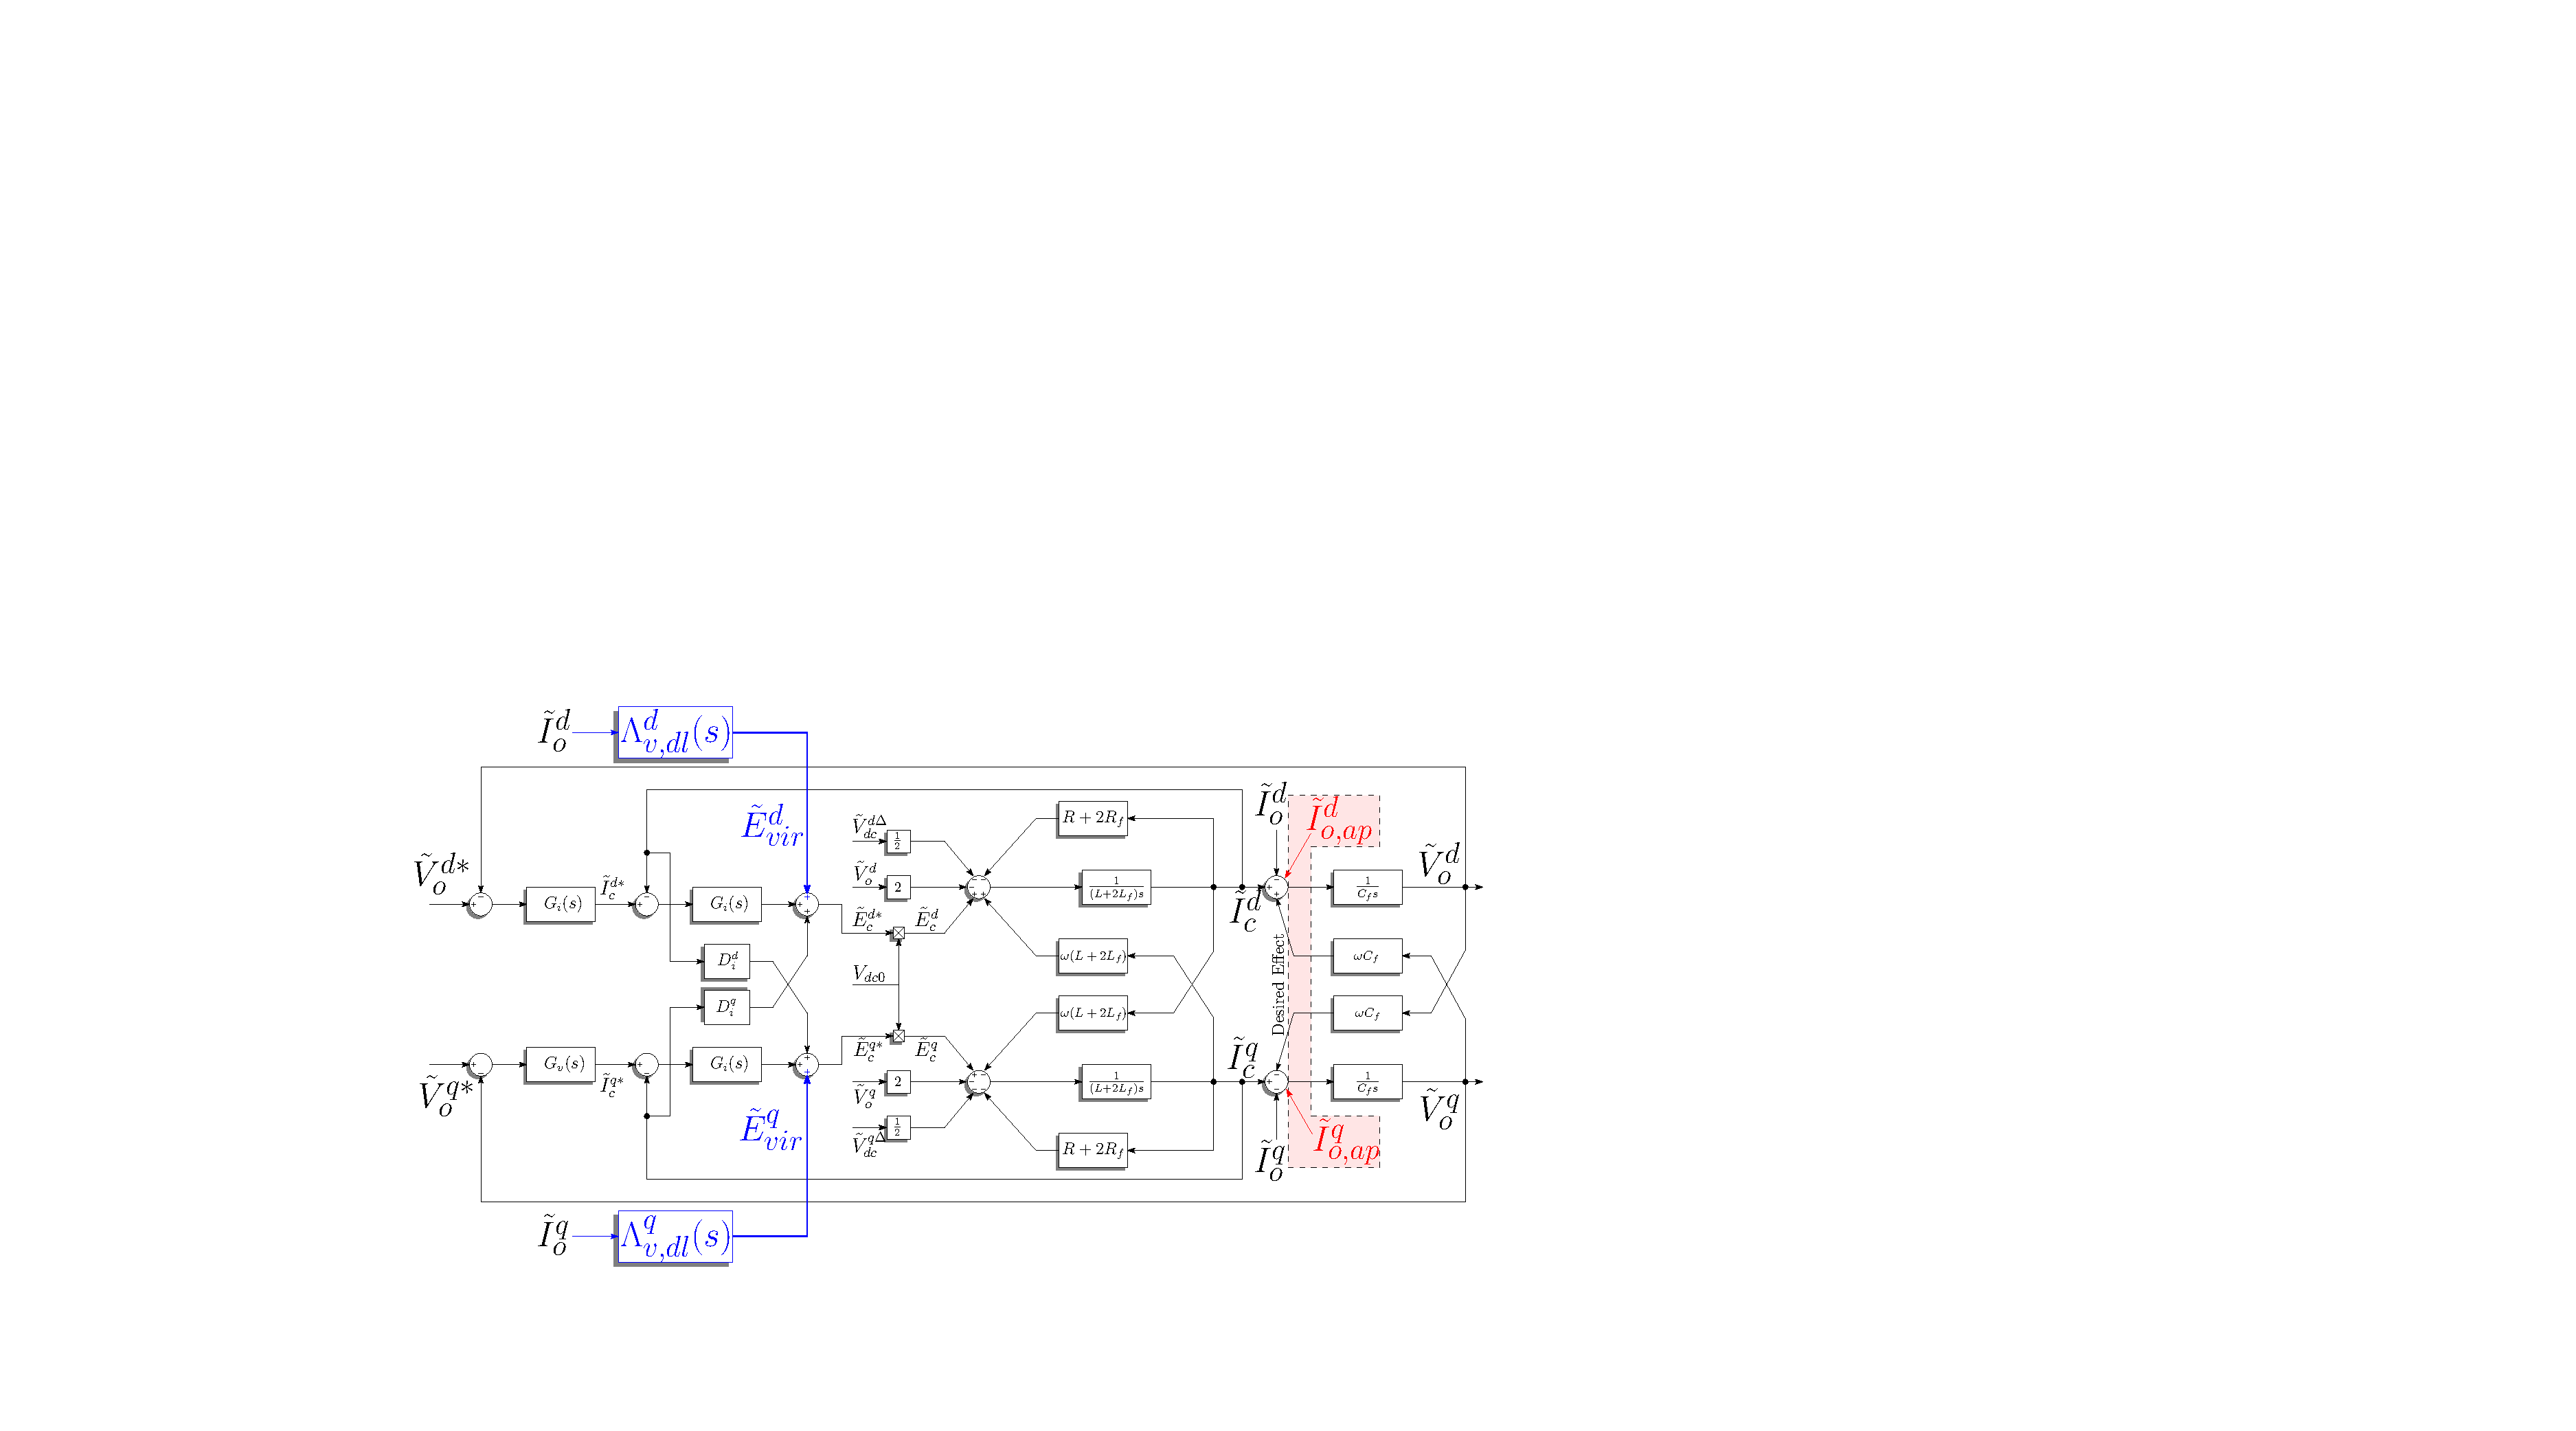
\includegraphics[width=0.95\linewidth]{./figuras/figuras_enhanced/block_diagram_SRF_icdq_Zvir_dl_3}

\end{columns}

%\vspace*{0.5cm}
{\color{blue}Ganho {\it feedforward}:} 
%
~~~~~~~~~~~~~~~~~~~~~~~~~~~~
%\tikz[baseline]{\node[anchor=west] (n1) {};}{\color{red!60}Filtro}
	\tikz[baseline]{
		\node[anchor=base] (n1)
			{\color{red}Filtro};
	}
%
\begin{equation*}
\vetorantpertctrlvdldqL  \approx 
\frac{1}{V_{dc0}}
\left[
	\tikz[baseline]{
		\node[fill=red!10,anchor=base] (t1)
			{$
				\frac{\omega_c }{s + \omega_c} 
			$};
	}s
\left(L + 2L_f\right)+
\left(R + 2R_f\right) 
\right]\mathbf{I}+
k_p^{i,dl} \mathbf{I} - \decidq
\end{equation*}


\begin{tikzpicture}[overlay]
        \path[->]<1-> (n1) edge [bend right,color=red] (t1);
\end{tikzpicture}

\end{frame}




%%%%%%%%%%%%%%%%%%%%%%%%%%%%%%%%%%%%%%%%%%%%%%%%%%%%%%%
%%%%%%%%%%%%%%%%%%%%%%%%%%%%%%%%%%%%%%%%%%%%%%%%%%%%%%%
%%%%%%%%%%%%%%%%%%%%%%%%%%%%%%%%%%%%%%%%%%%%%%%%%%%%%%%
\begin{frame}{Resultado}


\begin{columns}

\column{0.4\textwidth}
\centering

\begin{itemize}
	\item A parcela {\it feedforward} cria uma impedância virtual\\[15pt]
	
	\item Idealmente,\\[5pt] $|\vetorzvirdldqL(s)| = |\vetorzthdqL(s)|$ e\\[5pt] $\angle \vetorzvirdldqL(s) = - \angle \vetorzthdqL(s) $\\[15pt]
	
	\item O filtro impede esta condição ideal
\end{itemize}

\column{0.6\textwidth}
\centering

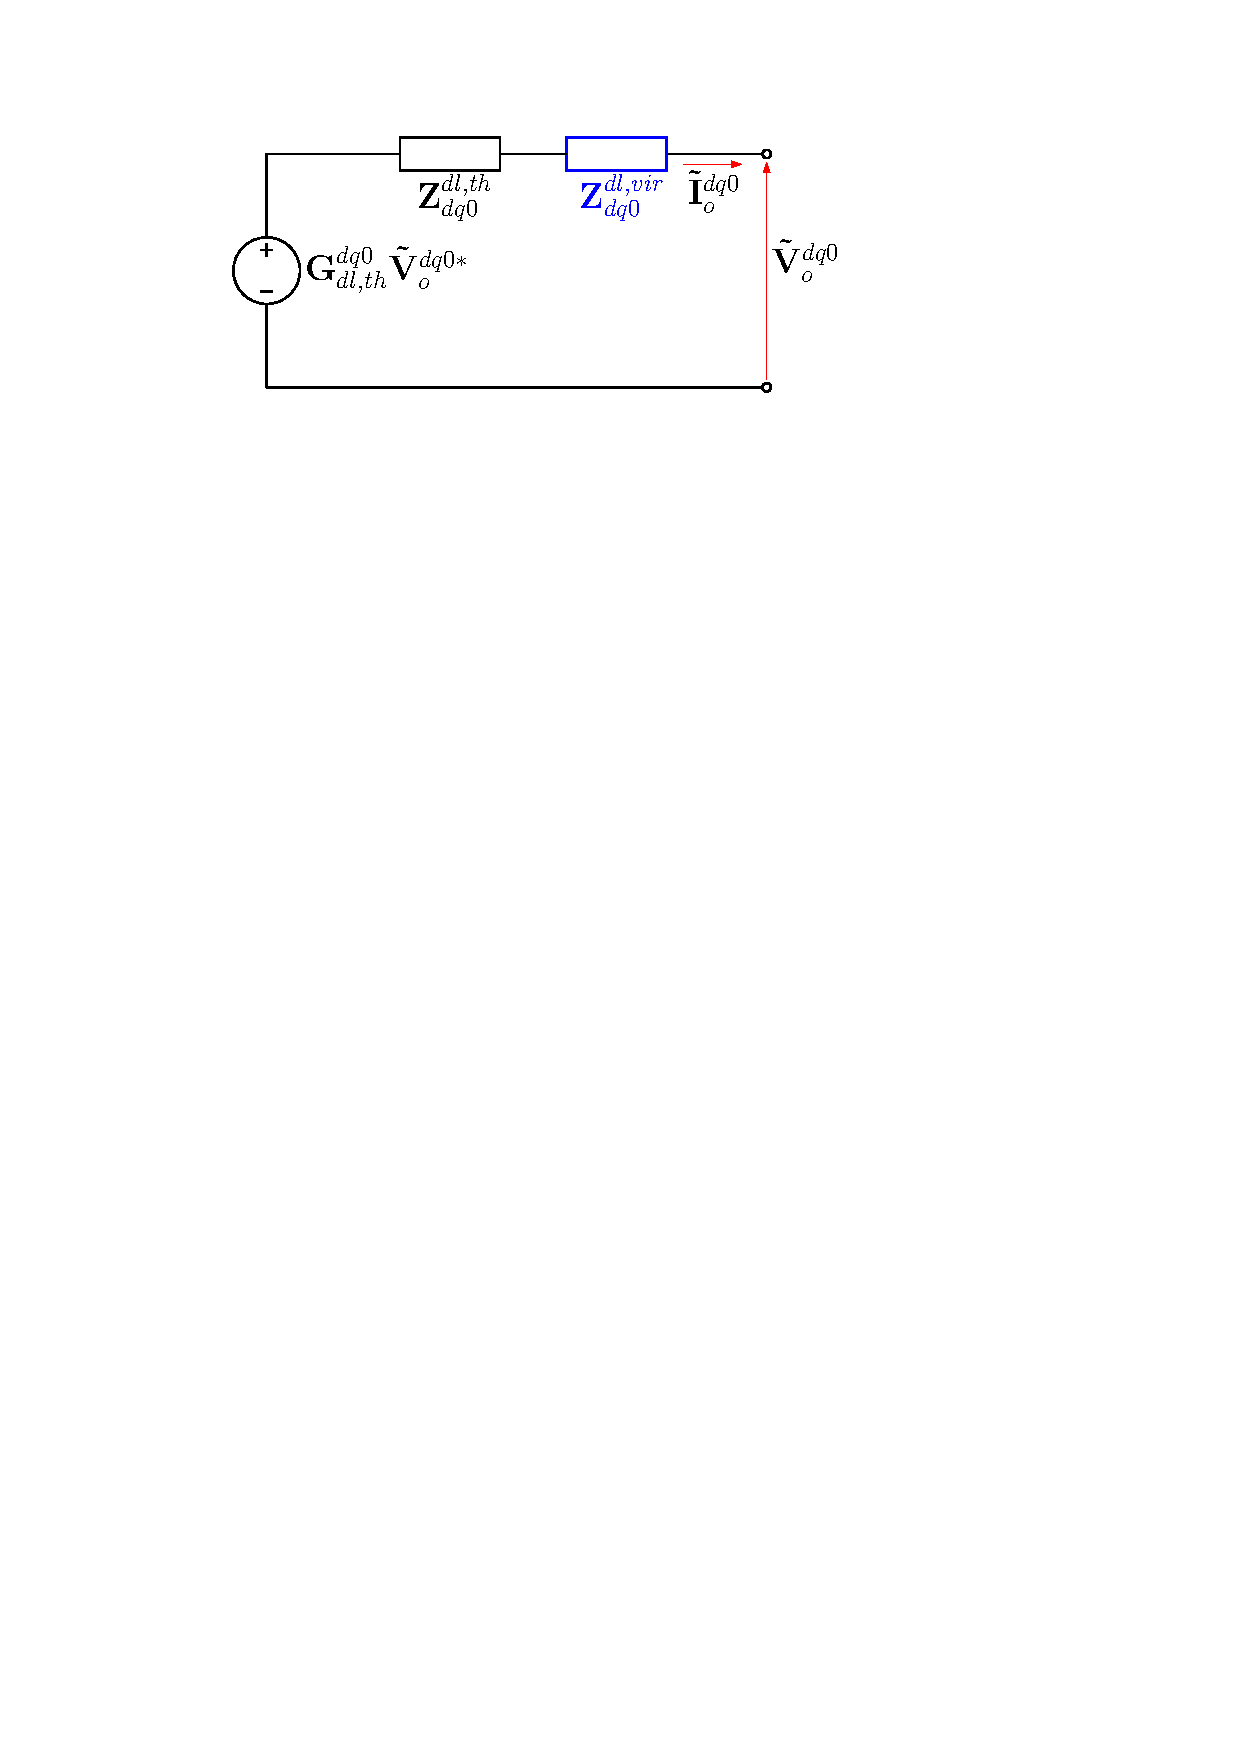
\includegraphics[width=0.9\linewidth]{./figuras/figuras_enhanced/Thevenin_SRF_VI_Zvir}



\begin{equation*}
\vetorzvirdldqL(s) = 
\vetorzthdqL(s)  \vetorgammavirsldqL(s)
\end{equation*}
%
\begin{equation*}
\resizebox{0.95\textwidth}{!} 
{$
\vetorgammavirsldqL (s) = - 
\vetorgichardqL^{-1}(s)
\left[
4 V_{dc0} C_{eq} \sdq + \frac{3S_0}{2 V_{dc0} } \mathbf{I}
\right]
\vetorantpertctrlvdldqL(s)
$}
\end{equation*}

\end{columns}







\end{frame}










%%%%%%%%%%%%%%%%%%%%%%%%%%%%%%%%%%%%%%%%%%%%%%%%%%%%%%%
%%%%%%%%%%%%%%%%%%%%%%%%%%%%%%%%%%%%%%%%%%%%%%%%%%%%%%%
%%%%%%%%%%%%%%%%%%%%%%%%%%%%%%%%%%%%%%%%%%%%%%%%%%%%%%%
\begin{frame}{Resultados de Simulação}



\begin{columns}

\column{0.75\textwidth}
\centering

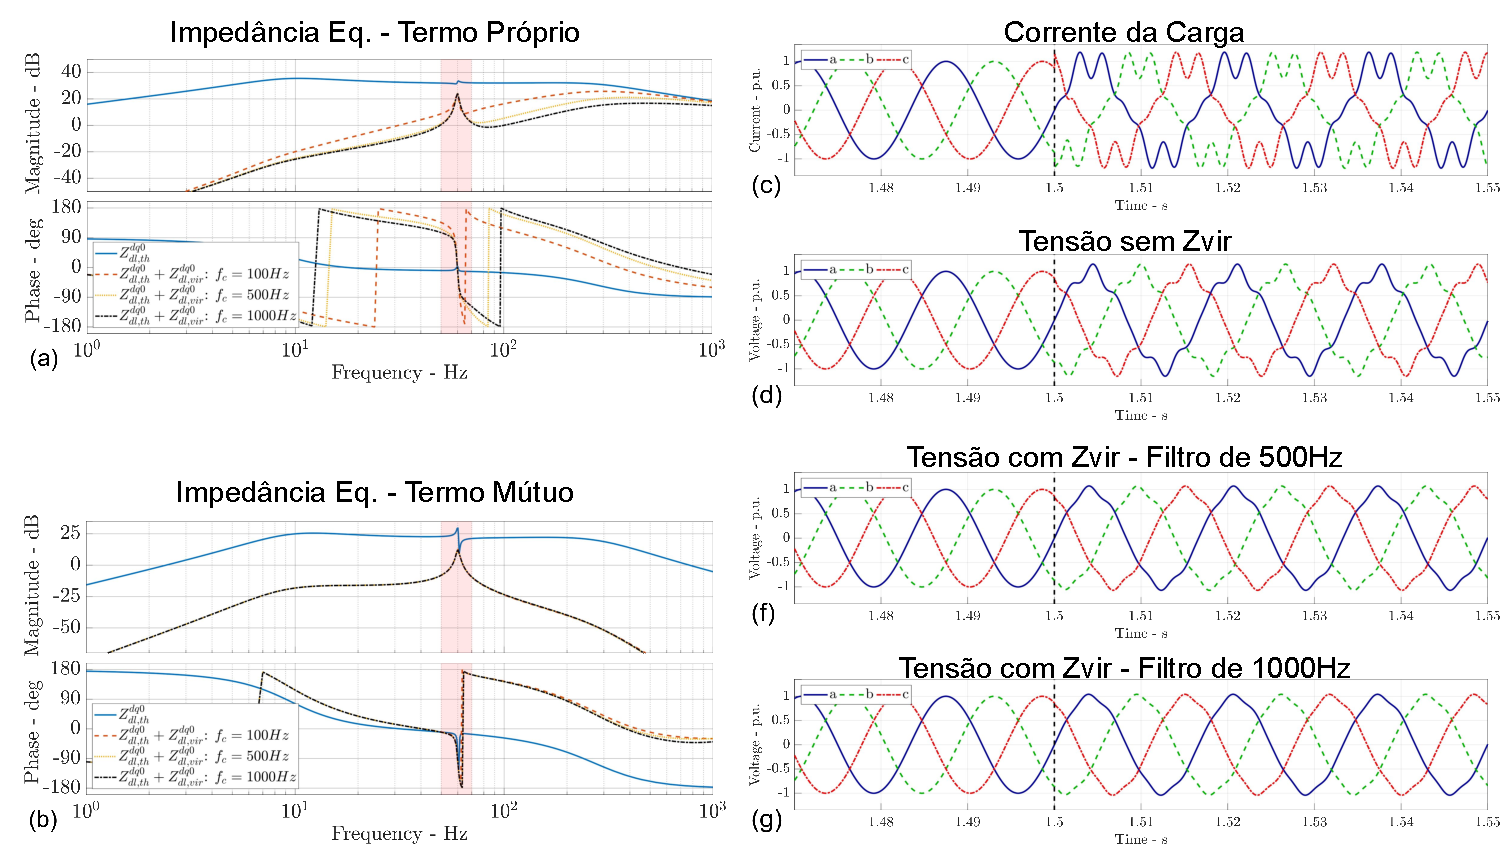
\includegraphics[width=1\linewidth]{./figuras/figuras_enhanced/slides_zvir_2}

\column{0.25\textwidth}
\centering



$\mathbf{Z}_{eq} = \vetorzvirdldqL + \vetorzthdqL$\\[10pt]



\end{columns}





\end{frame}

